% -*- root: ./report.tex -*-
\chapter{Methods}


\comment{We propose a method to verify that elimination of long trajectories is responsible for the increased topological gap in a zigzag system.}
\section{Quasiclassical estimation of the topological gap}
	\comment{To compute the effect of cutoff consider a single segment of the zigzag and obtain the spectrum analytically (this allows to use translation invariance).}
	In order to establish that the elimination of long trajectories is the driving mechanism behind the order of magnitude gap improvement, we use an analytical approach.
	We estimate the gap of the zigzag system by the minimum energy occuring in the Andreev spectrum of a single (diagonal) segment of zigzag.
	The spectrum of the zigzag segment we define as the spectrum of an infinite ribbon SNS junction with tilted-magnetic field. 
	The finite length of the segment is modeled by not including momenta corresponding to long trajectories when taking the minimum over the spectrum.

	\comment{The spectrum is derived using a scattering matrix, and we consider multiple ways to eliminate long trajectory momenta.}

	Estimating the gap is a two-step process: derivation of the Andreev spectrum, and taking the minimum energy over a particular set of allowed momenta.
	The first is derived using scattering matrix formalism and the Andreev bound state condition\cite{beenakker1991universal, sticlet_robustness_2017}.
	The second step is mostly trivial, but the difficulty lies with identifying the set of allowed  momenta to take the minimum over.


	\subsection{Analytical estimate of Andreev spectrum for a straight junction}
		
		We derive the spectrum by calculating the scattering matrix for the normal region and applying the Andreev bound state condition for the short junction limit\cite{beenakker1991universal, sticlet_robustness_2017}. 
		The short junction limit is valid for [TODO: WHEN IS THE SHORT JUNCTION LIMIT VALID]
		For deriviation of the scattering matrix, we neglect SOI in the transverse direction, which is valid for $W<l_\text{so}$.

		\subsubsection{Derivation of the scattering matrix}

			\begin{figure}[!htb]
			\includegraphics[width=0.95\columnwidth]{images/scattering}
			\caption{Basis for scattering matrix. 
			The `S' region corresponds to the superconductor Hamiltonian without the superconducting term, Eq.~\eqref{eq:ham_smat_superconducting}, `N' to the normal region, Eq.~\eqref{eq:ham_smat_normal}. 
			The coefficients represent the amplitude of the modes present in the system, at a particular energy.
			The different color arrows correspond to the two different spinors in each region.
			For example, $a_{1,L}$ is the amplitude of the rightmoving incoming mode, $\vec{\psi}_1 \exp\left(i k_{1,L} x\right)$}
			\label{fig:scattering}
			\end{figure}
			
			\begin{align}
			H_\text{N} &= \left[ \frac{\hbar^2}{2 \meff} \left(\kx^2 + \ky^2\right) -\mu_n\right]\sigi +
						 \alpha \kx \sigy +
						 E_z \left[ \cos(\theta) \sigx + \sin(\theta) \sigy \right]
			\label{eq:ham_smat_normal} \\
			H_\text{S} &= \left[\frac{\hbar^2}{2 \meff} \left(\kx^2 + \ky^2\right) -\mu_s\right]\sigi
			\label{eq:ham_smat_superconducting}
			\end{align}
			
			We consider the scattering region as depicted in Fig. \ref{fig:scattering}.
			There are three regions in the system, one normal system (N), with Hamiltonian given by Eq.~\eqref{eq:ham_smat_superconducting}, and two superconducting regions (S), with Hamiltonian given by Eq.~\eqref{eq:ham_smat_superconducting}.
			Not that Eq.~\eqref{eq:ham_smat_superconducting} region does not include the superconducting term ($\Delta \tau_y$), because we implement Andreev reflection seperately: this way we avoid doubling (electron and hole) the dimensionality of the problem.
			We set the energy of the system, and find the planar waves propogating in each region.
			Because the plane waves can go in two directions, and the additional degree of freedom introduced due to spin, each region has four propogating waves.
			The idea of the scattering matrix is to set the vector $\vec{a}$, containing the amplitudes of the planar waves coming in to the scattering region, and find the amplitudes of the modes exiting the scattering region.
			This is captured by a system of linear equations, displayed in Eq.~\eqref{eq:scattering_matrix_problem}
			
			\begin{equation}
			\begin{bmatrix} 
			b_{1,L}\\
			b_{2,L}\\
			b_{1,R}\\
			b_{2,R}
			\end{bmatrix} 
			= S_\text{sns}(\epsilon) \cdot 
			\begin{bmatrix} 
			a_{1,L}\\
			a_{2,L}\\
			a_{1,R}\\
			a_{2,R}
			\end{bmatrix}
			\label{eq:scattering_matrix_problem}
			\end{equation}

			In order to find the coefficients of the matrix $S_\text{sns}(\epsilon)$, we take the wavefunction $u(x)$ and apply the boundary equations (continuity and flux conservation): specified in Eqs.~\eqref{eq:scattering_equations} through \eqref{eq:scattering_boundary_eqs}.
			Note that because we neglect spin-orbit coupling in the x-direction, the velocity operator $\hat{\mathbf{v}}$ can be simplified to the first derivative.
			Although omitted to keep the expression compact, the momenta $k_i, q$ and spinors $\vec{\Psi_{i, L/R}}$ are energy dependent.

			\begin{align}
				&u(x) = 
				\begin{cases}
				u_L(x) = a_{1,L} \vec{\Psi} _{s,1} \exp (i q y) + a_{2,L} \vec{\Psi} _{s,2} \exp (i q y) + b_{1,L} \vec{\Psi} _{s,1} \exp (-i q y) + b_{2,L} \vec{\Psi} _{s,2} \exp (-i q y)  & x \leq 0\\
				u_m(x) = d_{1,l} \vec{\Psi} _{n,1} \exp \left(-i k_1 y\right) + d_{1,r} \vec{\Psi} _{n,1} \exp \left(i k_1 y\right) + d_{2,l} \vec{\Psi} _{n,2} \exp \left(-i k_2 y\right) + d_{2,r} \vec{\Psi} _{n,2} \exp \left(i k_2 y\right)  & 0 \geq x \leq W\\
				u_R(x) = a_{1,R} \vec{\Psi} _{s,1} \exp (-i q y) + a_{2,R} \vec{\Psi} _{s,2} \exp (-i q y) + b_{1,R} \vec{\Psi} _{s,1} \exp (i q y) + b_{2,R} \vec{\Psi} _{s,2} \exp (i q y)  & W \geq x
				\end{cases}
				\label{eq:scattering_equations}
			\end{align}
				
			Where $a_{i, L/R}$ are the coefficients of the incoming modes, $b_{i, L/R}$ are those of the outgoing modes, and $d_{i, l/r}$ are the modes in the middle region: see Fig.\ref{fig:scattering}.
			The symbols $\vec{\Psi}_{n/s, i}$ and $k_i, q$ are respectively the spinors and corresponding momenta belonging to each region.
			Both are energy dependent.\\

			The boundary conditions are,
			\begin{align}
				& u(x) \text{ is continuous}\\
				&\hat{\mathbf{v}} u(x) \text{ is continuous, where $\hat{\mathbf{v}}$ is the velocity operator}\label{eq:scattering_boundary_eqs}
			\end{align}

			To solve the system analytically, we use the Short Junction limit: we set the energy to zero.
			By applying the boundary conditions and solving the resulting linear system of equations, the resulting solution is given by Eqs.~\eqref{eq:smatrix} through ~\eqref{eq:momenta_short_junction}.
			\emph{Important note: In order to use the Andreev bound state condition, the scattering matrix must be in the [TODO: NAME OF BASIS] basis. This basis transformation has already been applied in Eqs. ~\eqref{eq:smatrix} through ~\eqref{eq:momenta_short_junction}}\\
			
			Scattering matrix, in block matrix format:
			\begin{align}
			\label{eq:smatrix}
		    S &= \left(
		    \begin{array}{rr}
		    r_{ll}&t_{rl}\\
		    t_{lr}&r_{rr}\\
		    \end{array}
		    \right) =
		    \left(
		    \begin{array}{rr}
		    \beta_+ & e^{-i q W} \beta_-\\
		    e^{-i q W} \beta_- & e^{-2 i q W} \beta_+\\
		    \end{array}
		    \right)
		    \\
		    \beta_\pm &= \left(
		    \begin{array}{rr}
		    e^{i \nu_{\arg}}\left(\omega^\pm_1 - \omega^\pm_2\right) & (\omega^\pm _1 + \omega^\pm _2)\\
		    -(\omega^\pm _1 + \omega^\pm _2) & e^{-i \nu _{\arg }} \left(\omega^\pm _2 - \omega^\pm _1\right)\\
		    \end{array}
		    \right)\\
		    \omega^\pm_j &= \frac{1}{4} \left(\gamma _{j} \pm \delta _{j}\right)
			\end{align}

			Subexpressions:
			\begin{align}
			    \gamma_j &= \frac{q+i k_{j} \tan \left(\frac{W k_{j}}{2}\right)}{q-i k_{j} \tan \left(\frac{W k_{j}}{2}\right)} \\
			    \delta_j &= \frac{q-i k_{j} \cot \left(\frac{W k_{j}}{2}\right)}{q+i k_{j} \cot \left(\frac{W k_{j}}{2}\right)}\\
			    e^{i \nu_{\arg}} &= \frac{E_\text{z} e^{i \theta }-i \alpha  k_x}{\sqrt{E_\text{z}^2+\alpha  k_x \left(\alpha  k_x-2 E_\text{z} \sin (\theta )\right)}}
			\end{align}

			Momenta:
			\begin{align}
			    q &= \left[ \frac{2 m_\ast}{\hbar ^2}\mu_s - k_x^2 \right]^\frac{1}{2}\\
			    k_1 &= \left[ \frac{2 m_\ast}{\hbar^2} \left(\mu_n-\sqrt{E_z^2-2 \alpha  E_z \sin (\theta ) k_x+\alpha ^2 k_x^2}\right) - k_x^2 \right]^\frac{1}{2}\\
			    k_2 &= \left[ \frac{2 m_\ast}{\hbar^2} \left(\mu_n+\sqrt{E_z^2-2 \alpha  E_z \sin (\theta ) k_x+\alpha ^2 k_x^2}\right) - k_x^2 \right]^\frac{1}{2}
			\label{eq:momenta_short_junction}
			\end{align}

		\subsubsection{Resulting spectrum}
			In order to get the spectrum from the S-matrix [Eq.~\eqref{eq:smatrix}] we use the main result from Ref.~\cite{beenakker1991universal} and start with a determinantal equation for the bound state energies in a SNS-junction:

			\begin{equation}
			\det\left[1+\alpha^{2}\left(E\right)r^{*}S_{e}\left(E,\bm{k}\right)rS_{e}^{*}\left(-E,-\bm{k}\right)\right]=0
			\end{equation}

			We rewrite this as a characteristic polynomial problem $\det\left[A-\lambda I\right]=0$, as

			\begin{equation}
			\det\left[r^{*}S_{e}\left(E,\bm{k}\right)rS_{e}^{*}\left(-E,-\bm{k}\right)-\frac{-1}{\alpha^{2}\left(E\right)}I\right]=0
			\end{equation}

			with
			\begin{equation}
			\lambda=-\frac{1}{\alpha^{2}\left(E\right)},\;A=r^{*}S_{e}\left(E,\bm{k}\right)rS_{e}^{*}\left(-E,-\bm{k}\right).
			\end{equation}

			Where $\lambda_i$ are the eigenvalues of $A$.
			Inverting $\alpha\left(E\right)\equiv\exp\left(-i\arccos\left(E/\Delta\right)\right)$ yields $\frac{E}{\Delta}=\frac{\alpha^{2}+1}{2\alpha}=\frac{1}{2}\left(\alpha+\alpha^{-1}\right)=\textrm{Re}(\alpha)$, where the last equality holds because $\alpha$ is unitary.
			Then, since $\alpha$ is only defined in the positive imaginary plane, the energies are $\frac{E_{i}}{\Delta}=\textrm{Re}\left(\sqrt{-1/\lambda_{i}}\right)$ where we take the root which has a positive imaginary part.
			Using this result and Eq.~\eqref{eq:smatrix}, we numerically find the Andreev spectrum.

	\subsection{Eliminating long trajectories}
		\comment{We devise two different ways to define the cutoff of momentum.}
			
		\begin{figure}[!htb]
		\centering
		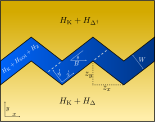
\includegraphics[width=0.75\columnwidth]{images/zigzag.pdf}
		\caption{Setups. Figure of a straight and zigzag system, including trajectories.
		\label{fig:setup}}
		\end{figure}
		
		\subsubsection{Momentum cutoff}
			We take the longest trajectory possible in a zigzag segment
		\subsubsection{Angular cutoff}


